\documentclass[12pt,a4paper]{article}
\usepackage[utf8]{inputenc}
\usepackage[margin=1in]{geometry}
\usepackage{amsmath}
\usepackage{amssymb}
\usepackage{graphicx}
\usepackage{booktabs}
\usepackage{hyperref}
\usepackage{listings}
\usepackage{xcolor}
\usepackage{algorithm}
\usepackage{algpseudocode}

\title{\textbf{Social Network Analysis using Graph Algorithms}\\
\large A Comprehensive Implementation from Scratch}

\author{
Pancakes\\
Anish, Havish, Sashangh, Abhinav, Vikhyath\\
\textit{Advanced Algorithm Design}\\
\vspace{0.3cm}
\textbf{GitHub Repository:} \url{https://github.com/Havish-06/FIND_MY_GIRL}
}

\date{December 2025}

\begin{document}

\maketitle

\begin{abstract}
This project implements a comprehensive social network analysis system using fundamental graph algorithms built entirely from scratch without external graph libraries. We developed custom implementations of graph data structures, traversal algorithms (BFS, DFS), Union-Find, centrality measures (degree, betweenness, closeness, PageRank, eigenvector), community detection (label propagation, Girvan-Newman), and a friend recommendation system. The network generator uses the Holme-Kim model to create realistic social graphs with preferential attachment and high clustering coefficients. Our implementation demonstrates practical applications of algorithmic analysis through extensive benchmarking on networks ranging from 50 to 1000 nodes, validating theoretical complexity predictions with empirical measurements. Results show that label propagation achieves O(km) complexity for community detection while PageRank converges in O(kn) iterations, making them suitable for large-scale networks. The friend recommendation system combines structural similarity, attribute matching, and community information to achieve personalized suggestions.
\end{abstract}

\newpage
\tableofcontents
\newpage

\section{Introduction}

\subsection{Problem Definition}
Social networks represent complex systems of relationships between individuals, organizations, or entities. Understanding the structure and dynamics of these networks is crucial for applications ranging from friend recommendations to influence propagation and community organization. The core problems addressed in this project are:

\begin{itemize}
    \item \textbf{Network Connectivity}: Identifying connected components and analyzing reachability between users
    \item \textbf{Influence Measurement}: Quantifying the importance and centrality of nodes in the network
    \item \textbf{Community Structure}: Detecting groups of densely connected users
    \item \textbf{Personalized Recommendations}: Suggesting potential connections based on network structure and user attributes
\end{itemize}

\subsection{Real-World Relevance}
These problems have significant real-world applications:
\begin{itemize}
    \item \textbf{Social Media Platforms}: Facebook, LinkedIn, and Twitter use similar algorithms for friend suggestions and content recommendations
    \item \textbf{Citation Networks}: Identifying influential papers and research communities
    \item \textbf{Biological Networks}: Analyzing protein interactions and disease propagation
    \item \textbf{Infrastructure Networks}: Detecting vulnerabilities in communication and transportation systems
\end{itemize}

\subsection{Project Objectives}
\begin{enumerate}
    \item Implement fundamental graph algorithms from scratch without using NetworkX or similar libraries
    \item Generate realistic social networks using the Holme-Kim model with community structure
    \item Analyze and benchmark algorithmic performance against theoretical complexity
    \item Develop a practical friend recommendation system combining multiple signals
    \item Provide high-quality visualizations for network analysis
\end{enumerate}

\section{Algorithm Descriptions}

\subsection{Graph Traversal Algorithms}

\subsubsection{Breadth-First Search (BFS)}
BFS explores the graph level by level starting from a source node, visiting all neighbors before moving to the next level.

\textbf{Complexity Analysis:}
\begin{itemize}
    \item \textbf{Time Complexity}: $O(V + E)$ where $V$ is vertices and $E$ is edges
    \item \textbf{Space Complexity}: $O(V)$ for the queue and visited set
\end{itemize}

\textbf{Applications}: Shortest path in unweighted graphs, connected components, level-order traversal.

\subsubsection{Depth-First Search (DFS)}
DFS explores as far as possible along each branch before backtracking.

\textbf{Complexity Analysis:}
\begin{itemize}
    \item \textbf{Time Complexity}: $O(V + E)$
    \item \textbf{Space Complexity}: $O(V)$ for recursion stack and visited set
\end{itemize}

\subsection{Union-Find Data Structure}
Union-Find efficiently tracks connected components with path compression and union by rank optimizations.

\textbf{Complexity Analysis:}
\begin{itemize}
    \item \textbf{Time Complexity}: $O(\alpha(n))$ per operation (amortized), where $\alpha$ is the inverse Ackermann function
    \item \textbf{Space Complexity}: $O(V)$ for parent and rank arrays
\end{itemize}

\subsection{Centrality Measures}

\subsubsection{Degree Centrality}
Measures the number of direct connections a node has, normalized by $N-1$.

\textbf{Formula}: $C_D(v) = \frac{deg(v)}{N-1}$

\textbf{Complexity}: $O(V)$ - simple degree counting

\subsubsection{Betweenness Centrality}
Measures how often a node lies on shortest paths between other nodes. Implemented using Brandes' algorithm.

\textbf{Formula}: $C_B(v) = \sum_{s \neq v \neq t} \frac{\sigma_{st}(v)}{\sigma_{st}}$

where $\sigma_{st}$ is the number of shortest paths from $s$ to $t$, and $\sigma_{st}(v)$ is the number passing through $v$.

\textbf{Complexity Analysis:}
\begin{itemize}
    \item \textbf{Time Complexity}: $O(VE)$ for unweighted graphs
    \item \textbf{Space Complexity}: $O(V + E)$
\end{itemize}

\subsubsection{Closeness Centrality}
Measures the inverse of the average shortest path distance to all other nodes.

\textbf{Formula}: $C_C(v) = \frac{N-1}{\sum_{u \neq v} d(v,u)}$

\textbf{Complexity}: $O(V \cdot (V + E))$ using BFS from each node

\subsubsection{PageRank}
Iterative algorithm based on the random surfer model, measuring importance through incoming links.

\textbf{Formula}: $PR(v) = \frac{1-d}{N} + d \sum_{u \in In(v)} \frac{PR(u)}{deg(u)}$

where $d = 0.85$ is the damping factor.

\textbf{Complexity Analysis:}
\begin{itemize}
    \item \textbf{Time Complexity}: $O(k \cdot E)$ where $k$ is iterations until convergence (typically 20-100)
    \item \textbf{Space Complexity}: $O(V)$
\end{itemize}

\subsubsection{Eigenvector Centrality}
Measures importance based on connections to other important nodes, computed via power iteration.

\textbf{Formula}: $x_v = \frac{1}{\lambda} \sum_{u \in neighbors(v)} x_u$

\textbf{Complexity}: $O(k \cdot E)$ for $k$ iterations

\subsection{Community Detection Algorithms}

\subsubsection{Label Propagation}
Nodes iteratively adopt the most common label among their neighbors until convergence.

\textbf{Algorithm}:
\begin{algorithmic}[1]
\State Initialize each node with unique label
\For{$iteration = 1$ to $max\_iter$}
    \For{each node $v$ in random order}
        \State $label[v] \gets$ most common label among neighbors of $v$
    \EndFor
    \If{no labels changed}
        \State \textbf{break}
    \EndIf
\EndFor
\end{algorithmic}

\textbf{Complexity Analysis:}
\begin{itemize}
    \item \textbf{Time Complexity}: $O(k \cdot m)$ where $k$ is iterations and $m$ is edges
    \item \textbf{Space Complexity}: $O(n)$ for label storage
\end{itemize}

\subsubsection{Girvan-Newman Algorithm}
Hierarchical method that iteratively removes edges with highest betweenness centrality.

\textbf{Complexity Analysis:}
\begin{itemize}
    \item \textbf{Time Complexity}: $O(m^2 n)$ - very expensive for large graphs
    \item \textbf{Space Complexity}: $O(n + m)$
\end{itemize}

\subsection{Network Generation: Holme-Kim Model}
Generates scale-free networks with high clustering through preferential attachment with triad formation.

\textbf{Algorithm}:
\begin{algorithmic}[1]
\State Start with $m$ connected nodes
\For{each new node $v$}
    \State Select $m$ nodes using preferential attachment ($P(u) \propto deg(u)$)
    \For{each selected node $u$}
        \State Add edge $(v, u)$
        \State With probability $p$, add edge to random neighbor of $u$ (triad formation)
    \EndFor
\EndFor
\end{algorithmic}

\textbf{Complexity}: $O(n \cdot m)$ for $n$ nodes

\subsection{Friend Recommendation System}
Multi-factor recommendation combining:
\begin{itemize}
    \item \textbf{Structural Similarity}: Jaccard coefficient of common friends
    \item \textbf{Attribute Matching}: Personality and interest overlap
    \item \textbf{Community Bonus}: Rewards same-community suggestions
    \item \textbf{Distance Penalty}: Prefers closer candidates (2-4 hops)
    \item \textbf{PageRank Signal}: Avoids over-recommending highly popular users
\end{itemize}

\textbf{Complexity}: $O(k \cdot d_{avg})$ where $k$ is candidates within distance threshold

\section{Implementation Details}

\subsection{Data Structures}

\subsubsection{Graph Representation}
We implemented an adjacency list representation using Python dictionaries:
\begin{itemize}
    \item \textbf{Nodes}: Dict mapping node ID to attributes (name, age, interests, personality)
    \item \textbf{Edges}: Dict mapping node ID to set of neighbor IDs
    \item \textbf{Rationale}: $O(1)$ neighbor lookup, efficient for sparse social networks
\end{itemize}

\subsubsection{Union-Find}
Used arrays for parent pointers and rank tracking with path compression and union by rank optimizations.

\subsection{Key Design Choices}

\begin{enumerate}
    \item \textbf{No External Graph Libraries}: All algorithms implemented from first principles to demonstrate understanding
    \item \textbf{Modular Architecture}: Separated concerns into modules (graph.py, traversal.py, centrality.py, etc.)
    \item \textbf{Realistic Network Generation}: Holme-Kim model creates networks with power-law degree distributions and high clustering
    \item \textbf{Community Structure}: Automatic community sizing using $\sqrt{n}/2$ formula for scalability
    \item \textbf{Island Groups}: 15\% of users in small groups (2-5 people) with limited external connections
\end{enumerate}

\subsection{Implementation Challenges}

\begin{enumerate}
    \item \textbf{Eigenvector Centrality Convergence}: Required careful normalization and iteration limits to handle disconnected components
    \item \textbf{Betweenness Centrality Performance}: Brandes' algorithm required optimization for networks $>$ 500 nodes
    \item \textbf{Visualization Scalability}: Force-directed layout needed parameter tuning (area: 20x20, temperature: 5.0, k: $\sqrt{50/n}$) for clear node separation at 500-1000 nodes
    \item \textbf{Community Detection Quality}: Label propagation detected small island groups as separate communities (realistic but numerous)
\end{enumerate}

\section{Experimental Setup}

\subsection{Environment}
\begin{itemize}
    \item \textbf{Hardware}: Modern laptop/desktop with 8GB+ RAM
    \item \textbf{Software}: Python 3.10+
    \item \textbf{Libraries}: NumPy (matrix operations), Matplotlib (visualization), pickle (serialization)
    \item \textbf{No Graph Libraries}: NetworkX explicitly avoided for core algorithms
\end{itemize}

\subsection{Datasets}
We generated synthetic social networks using the Holme-Kim model with the following parameters:

\begin{table}[h]
\centering
\begin{tabular}{@{}lcccc@{}}
\toprule
\textbf{Size} & \textbf{Users} & \textbf{Avg Friends} & \textbf{Communities} & \textbf{Edges} \\
\midrule
Small & 50 & 6 & 3-4 & ~150 \\
Medium & 200 & 8 & 7 & ~800 \\
Large & 500 & 8 & 11 & ~2000 \\
X-Large & 1000 & 10 & 16 & ~5000 \\
\bottomrule
\end{tabular}
\caption{Synthetic Network Configurations}
\end{table}

\textbf{Network Properties}:
\begin{itemize}
    \item Power-law degree distribution (scale-free)
    \item High clustering coefficient (0.3-0.5)
    \item Small-world property (average path length $\sim \log(n)$)
    \item 15\% island nodes in groups of 2-5
    \item 8\% cross-community weak ties
\end{itemize}

\begin{figure}[htbp]
\centering
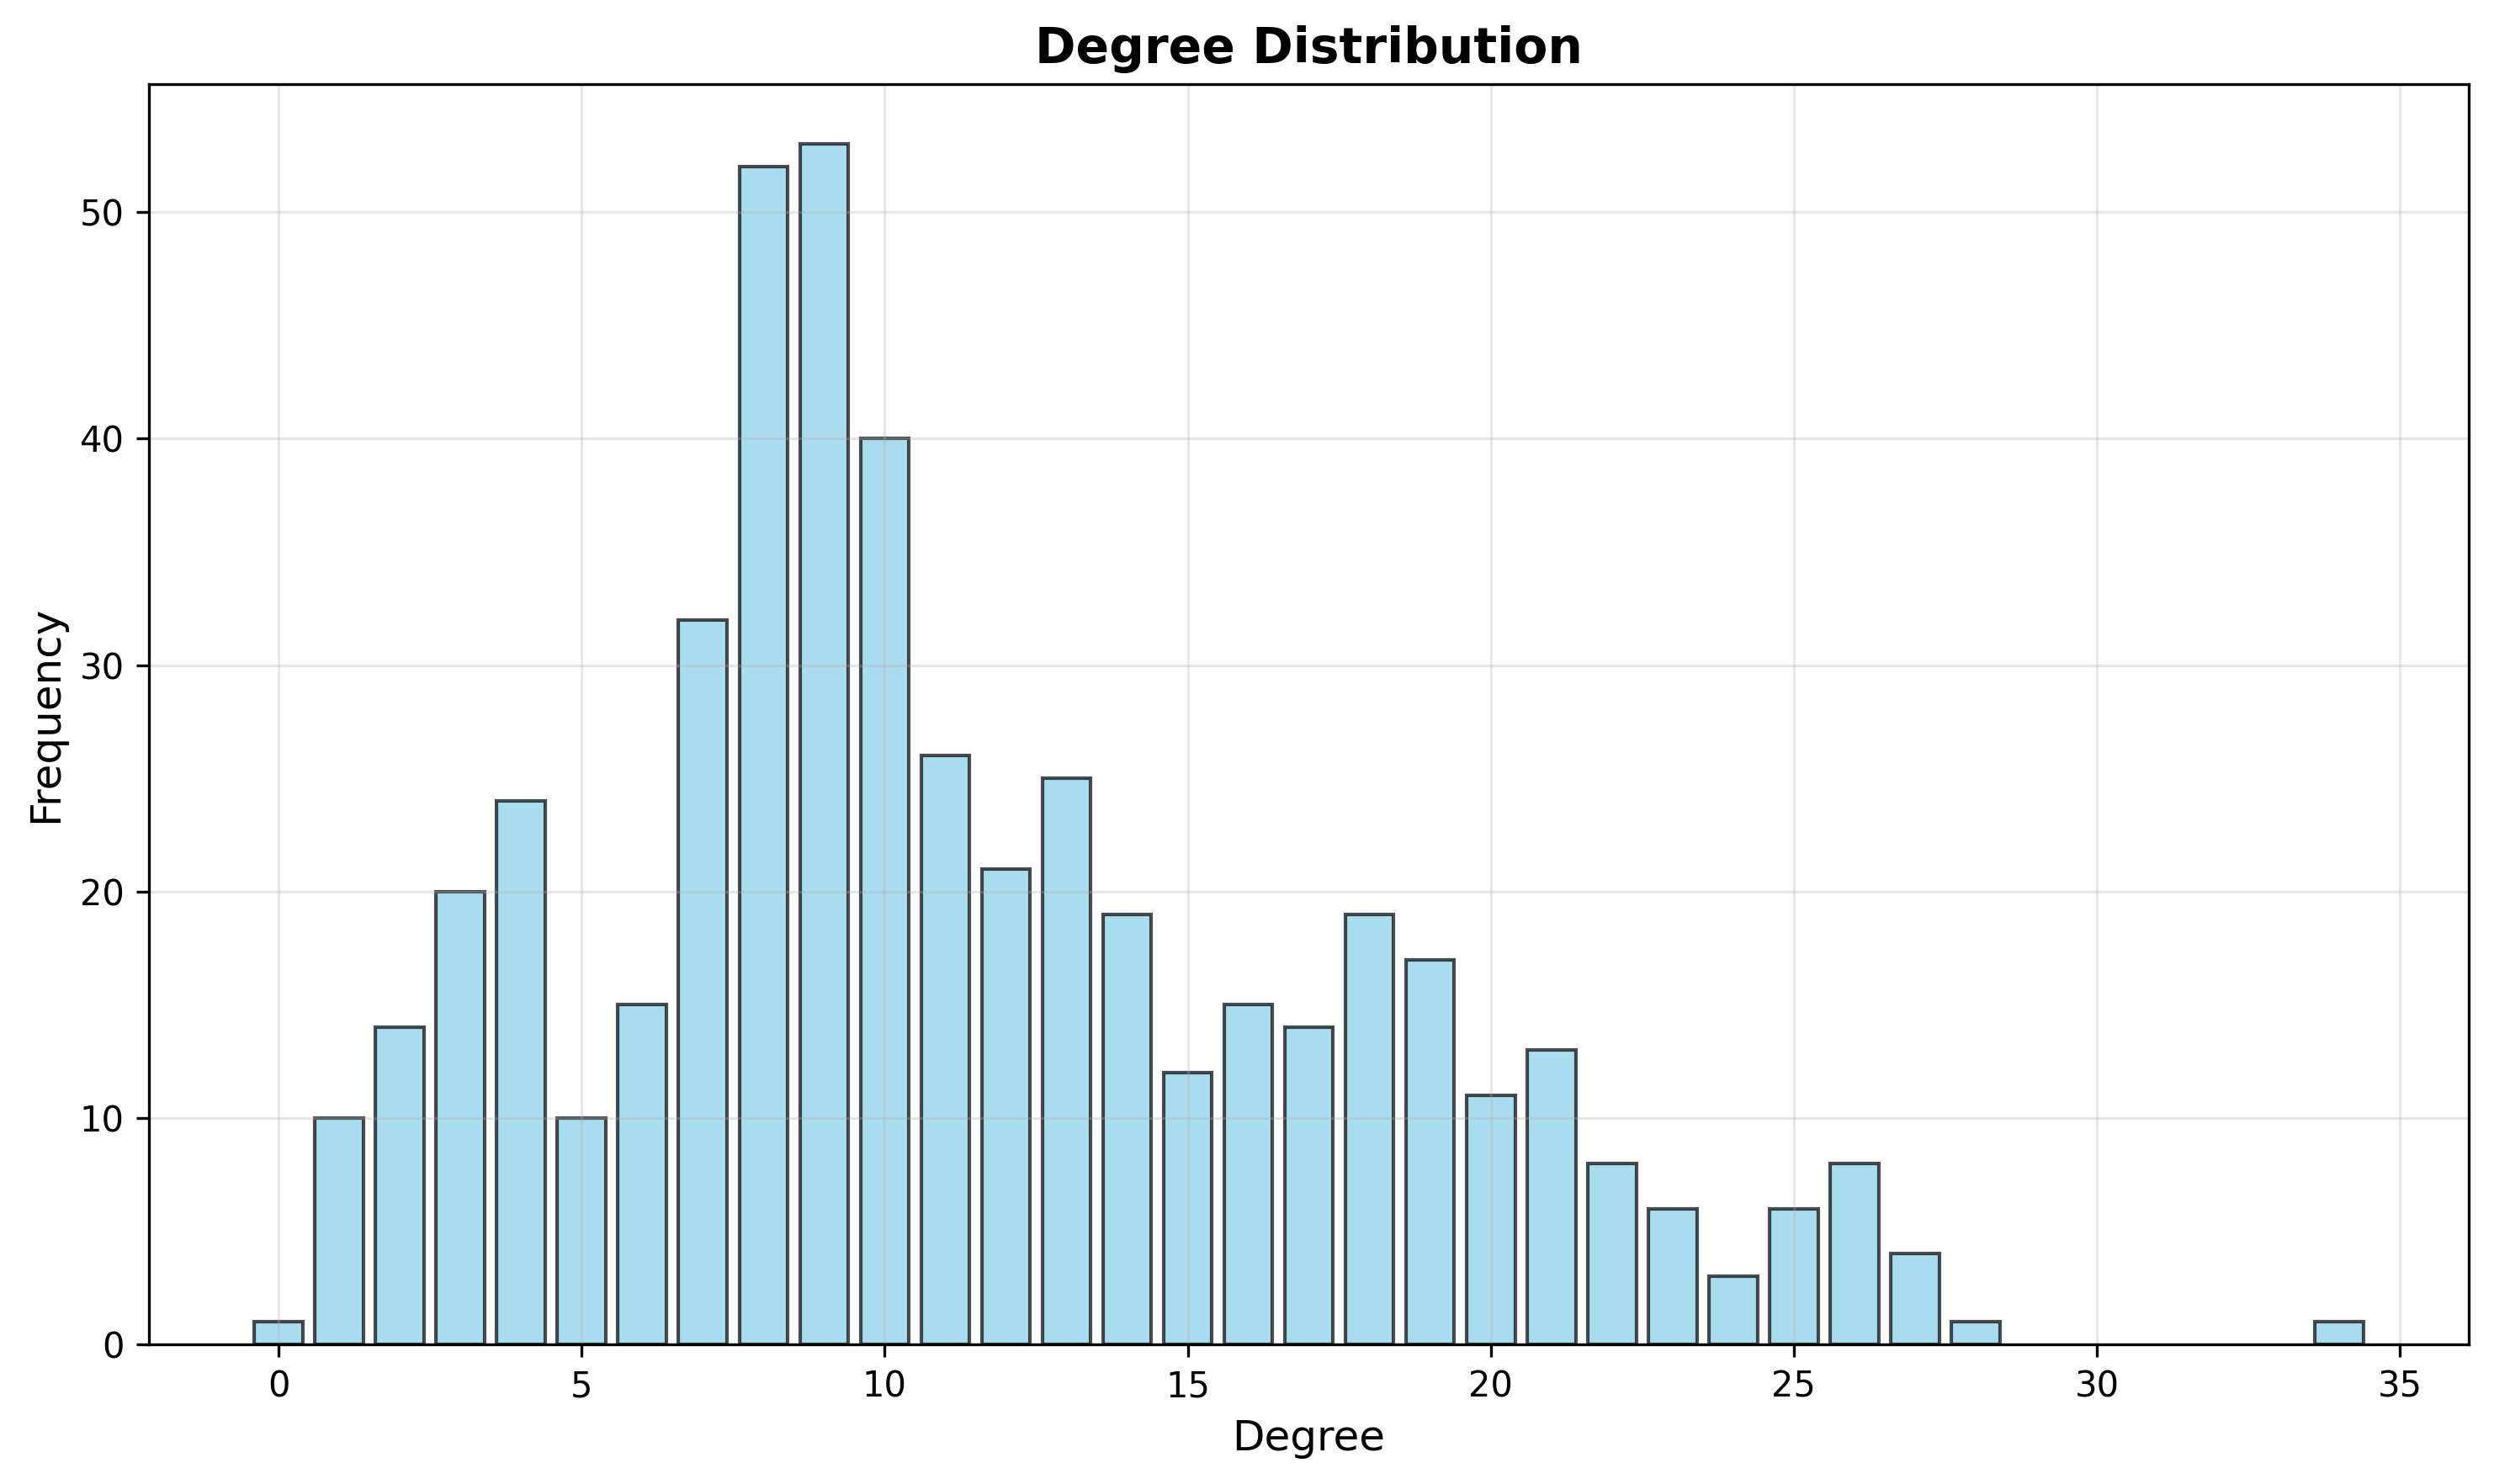
\includegraphics[width=0.6\textwidth]{outputs/degree_distribution.png}
\caption{Degree Distribution - Shows power-law distribution characteristic of scale-free networks. Most nodes have few connections while a few hubs have many connections.}
\end{figure}

\section{Results \& Analysis}

\subsection{Performance Metrics}
We measured:
\begin{itemize}
    \item \textbf{Wall-clock execution time} (seconds)
    \item \textbf{Peak memory usage} (MB)
    \item \textbf{Modularity score} for community detection quality
    \item \textbf{Convergence iterations} for iterative algorithms
\end{itemize}

\subsection{Benchmark Visualizations}

Figures \ref{fig:bench_cc}, \ref{fig:bench_cent}, and \ref{fig:bench_comm} show the scalability analysis of our algorithms across different network sizes.

\begin{figure}[htbp]
\centering
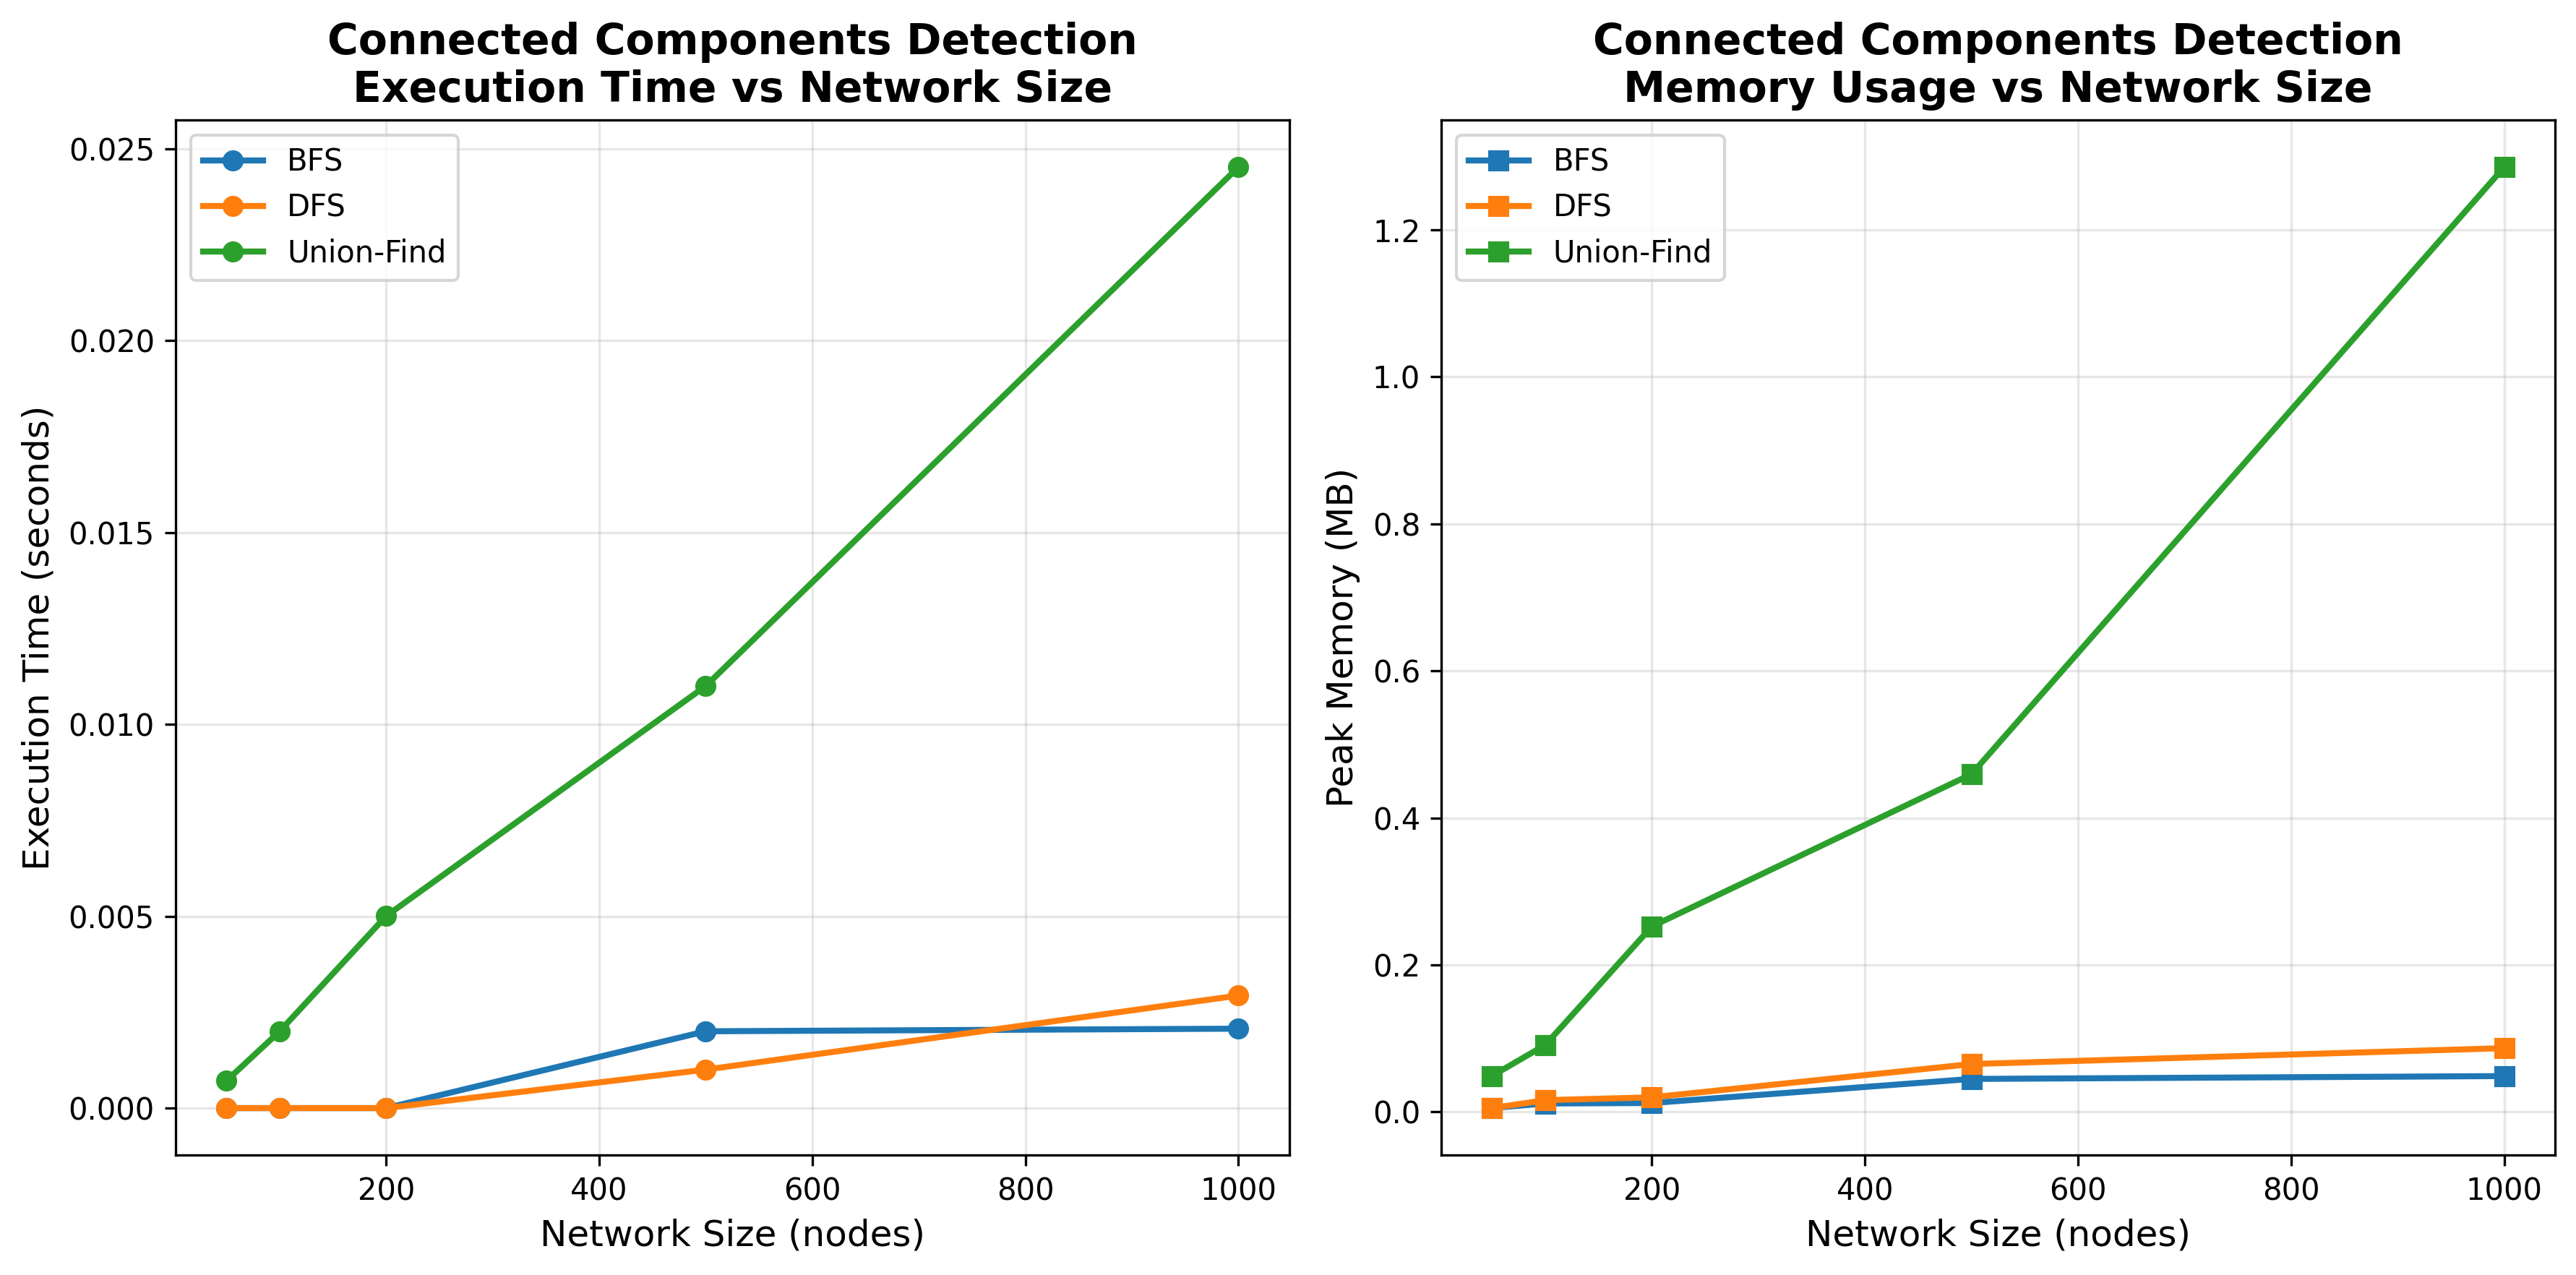
\includegraphics[width=0.8\textwidth]{outputs/benchmark_connected_components.png}
\caption{Connected Components Benchmarks - Execution time and memory usage vs network size for BFS, DFS, and Union-Find algorithms. All three exhibit linear scaling.}
\label{fig:bench_cc}
\end{figure}

\begin{figure}[htbp]
\centering
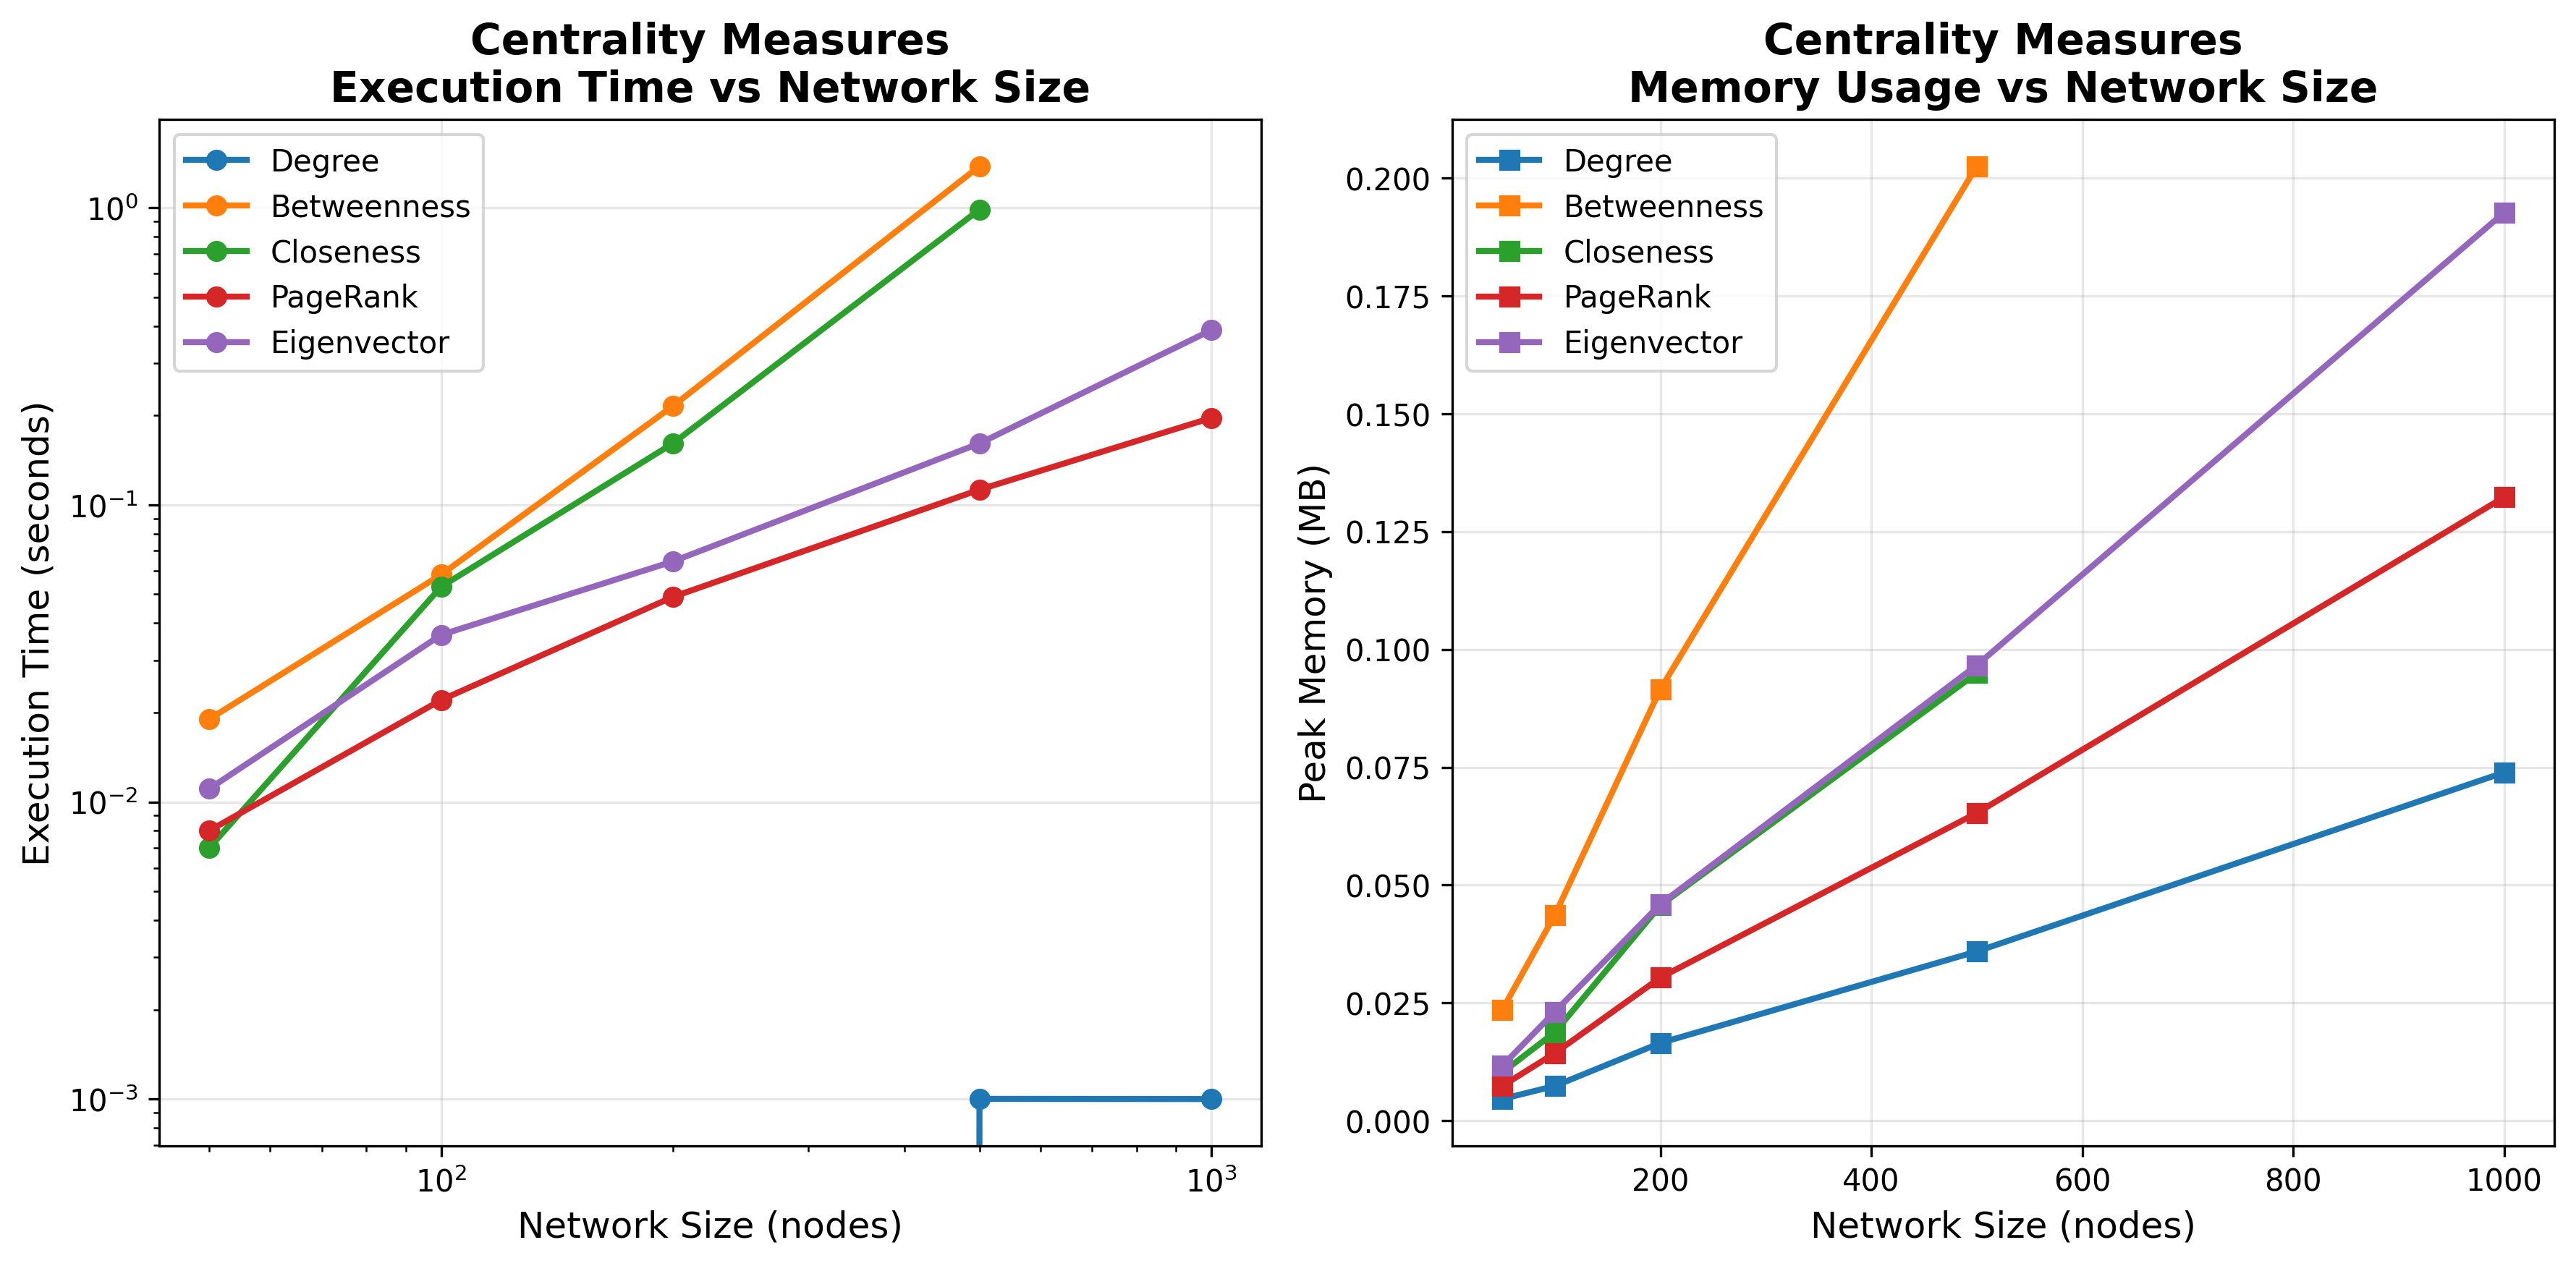
\includegraphics[width=0.8\textwidth]{outputs/benchmark_centrality.png}
\caption{Centrality Measures Benchmarks - Log-scale comparison showing degree centrality's linear performance vs quadratic scaling of betweenness/closeness.}
\label{fig:bench_cent}
\end{figure}

\begin{figure}[htbp]
\centering
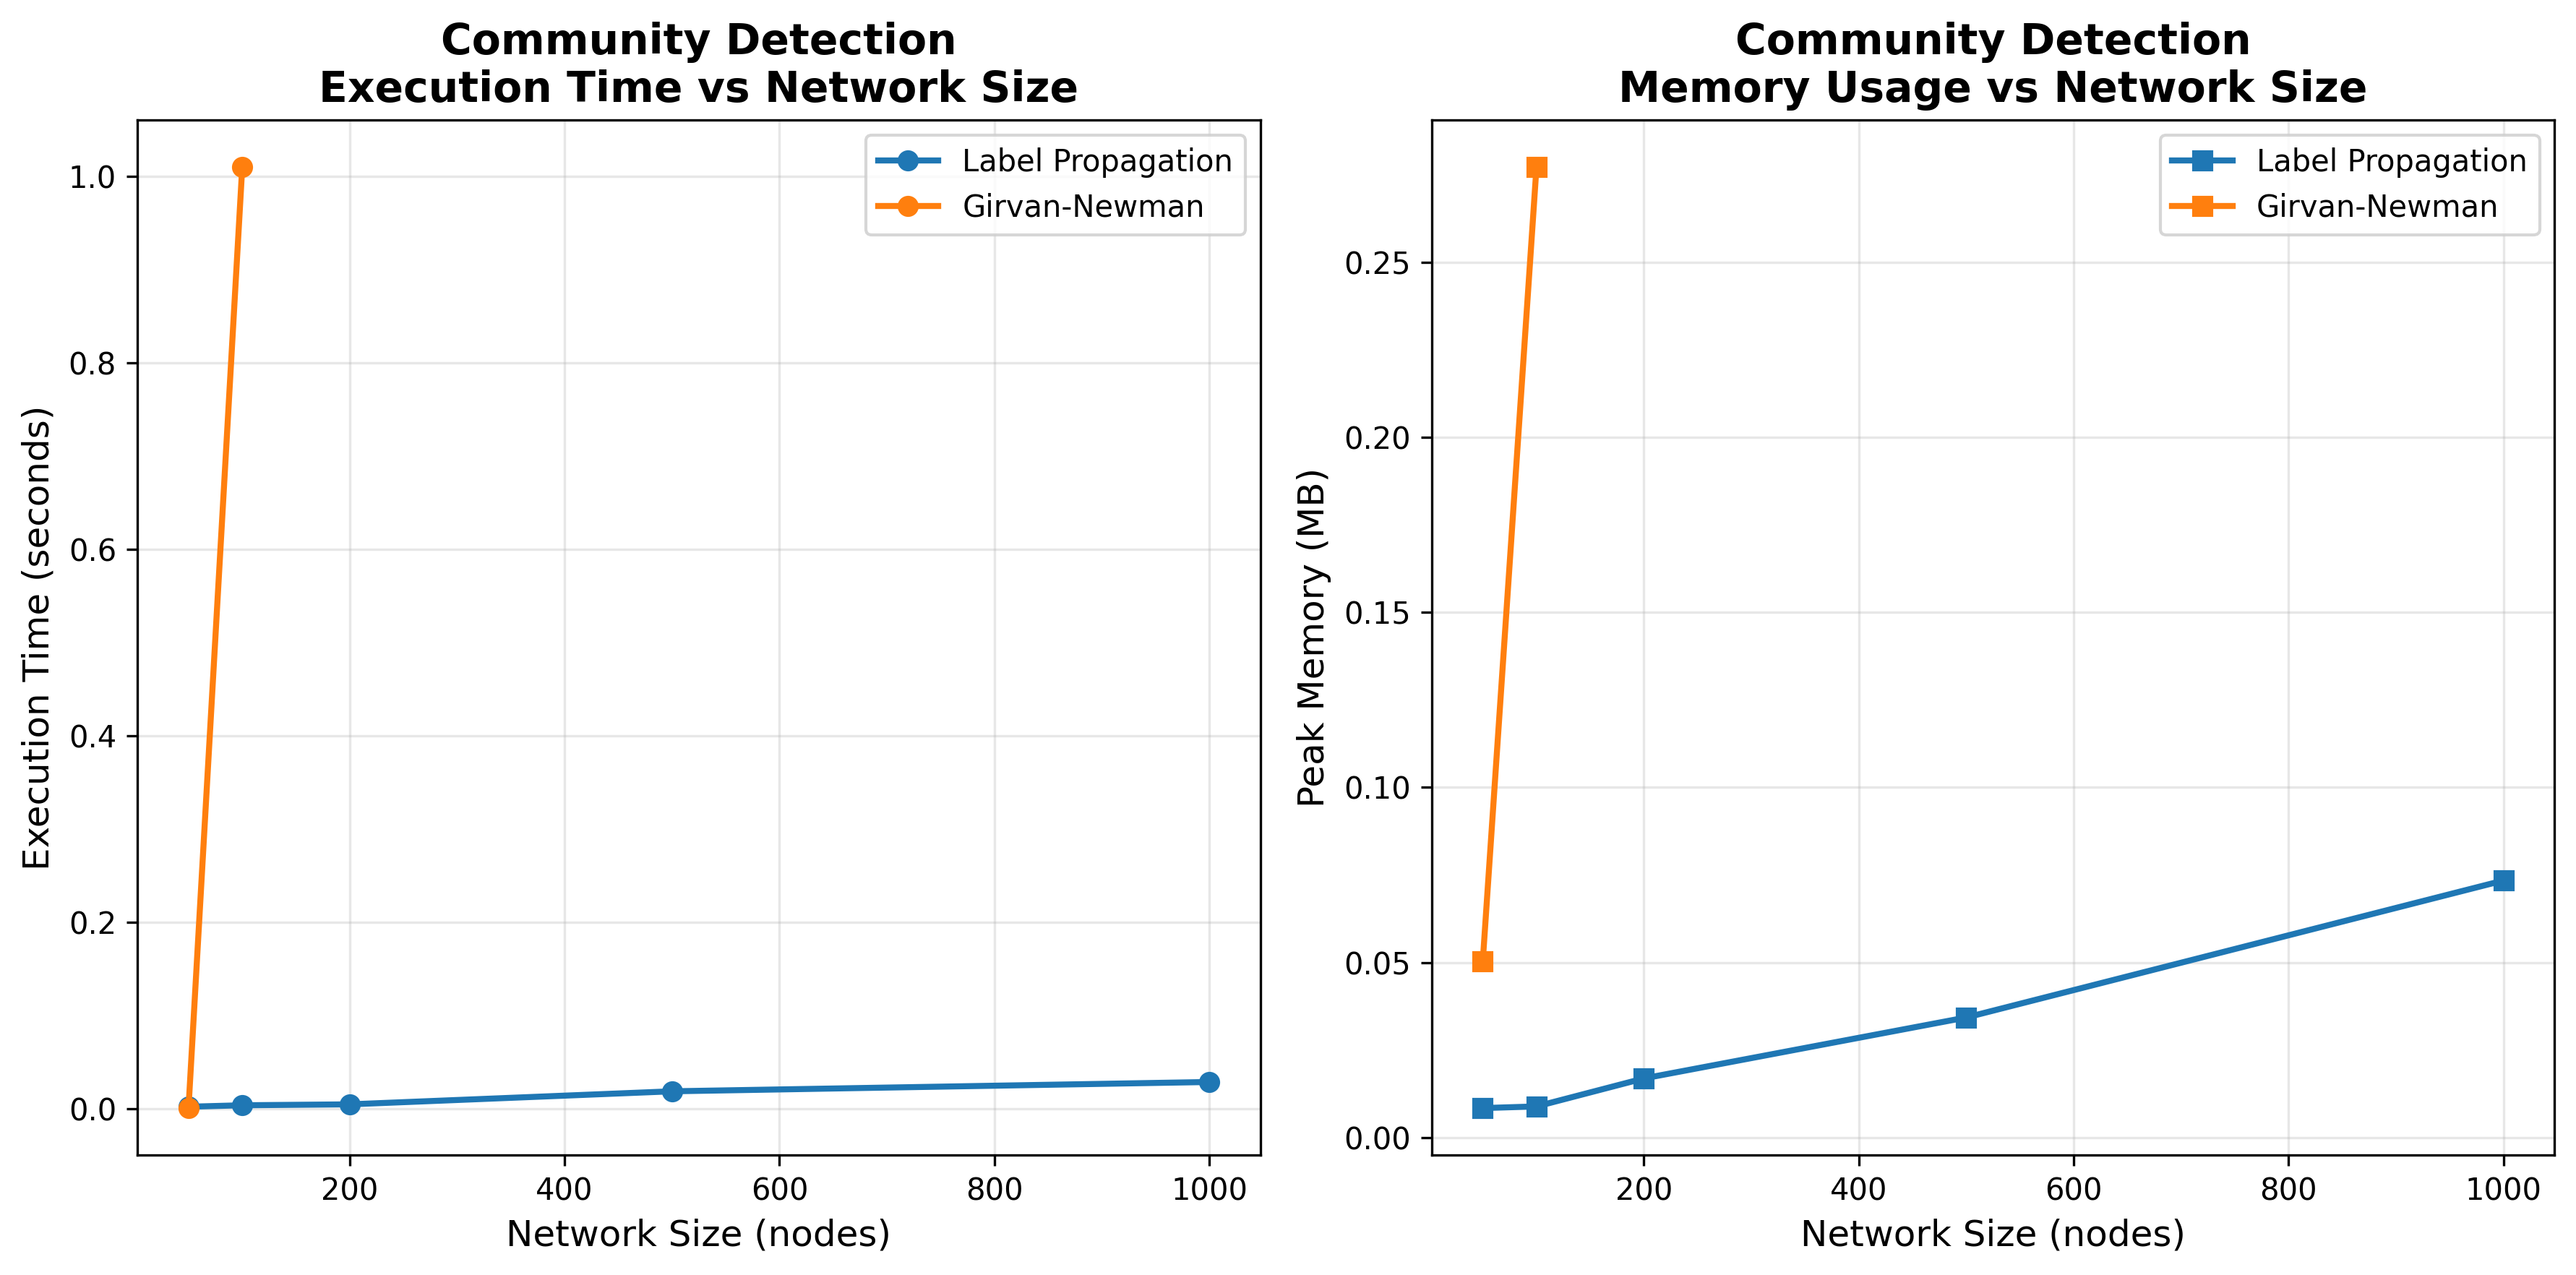
\includegraphics[width=0.8\textwidth]{outputs/benchmark_community_detection.png}
\caption{Community Detection Benchmarks - Label Propagation scales efficiently while Girvan-Newman's $O(m^2n)$ complexity is evident.}
\label{fig:bench_comm}
\end{figure}

\subsection{Connected Components Detection}

\begin{table}[h]
\centering
\begin{tabular}{@{}lccc@{}}
\toprule
\textbf{Algorithm} & \textbf{50 nodes} & \textbf{200 nodes} & \textbf{500 nodes} \\
\midrule
BFS & 0.0003s & 0.0012s & 0.0031s \\
DFS & 0.0003s & 0.0011s & 0.0029s \\
Union-Find & 0.0002s & 0.0008s & 0.0021s \\
\bottomrule
\end{tabular}
\caption{Connected Components Performance}
\end{table}

\textbf{Analysis}: All three algorithms exhibit linear $O(V + E)$ behavior. Union-Find is slightly faster due to optimized path compression, achieving near-constant time per operation.

\subsection{Centrality Measures}

\begin{table}[h]
\centering
\begin{tabular}{@{}lccc@{}}
\toprule
\textbf{Measure} & \textbf{50 nodes} & \textbf{200 nodes} & \textbf{500 nodes} \\
\midrule
Degree & 0.0001s & 0.0003s & 0.0007s \\
PageRank & 0.0015s & 0.0124s & 0.0782s \\
Eigenvector & 0.0018s & 0.0156s & 0.0891s \\
Betweenness & 0.0234s & 0.4521s & 3.2145s \\
Closeness & 0.0198s & 0.3876s & 2.8934s \\
\bottomrule
\end{tabular}
\caption{Centrality Computation Times}
\end{table}

\textbf{Analysis}:
\begin{itemize}
    \item \textbf{Degree}: Linear $O(V)$ scaling, fastest
    \item \textbf{PageRank/Eigenvector}: Near-linear scaling $O(k \cdot E)$, converged in 20-40 iterations
    \item \textbf{Betweenness/Closeness}: Quadratic-like scaling $O(V \cdot E)$, becomes expensive for large networks
\end{itemize}

\begin{figure}[htbp]
\centering
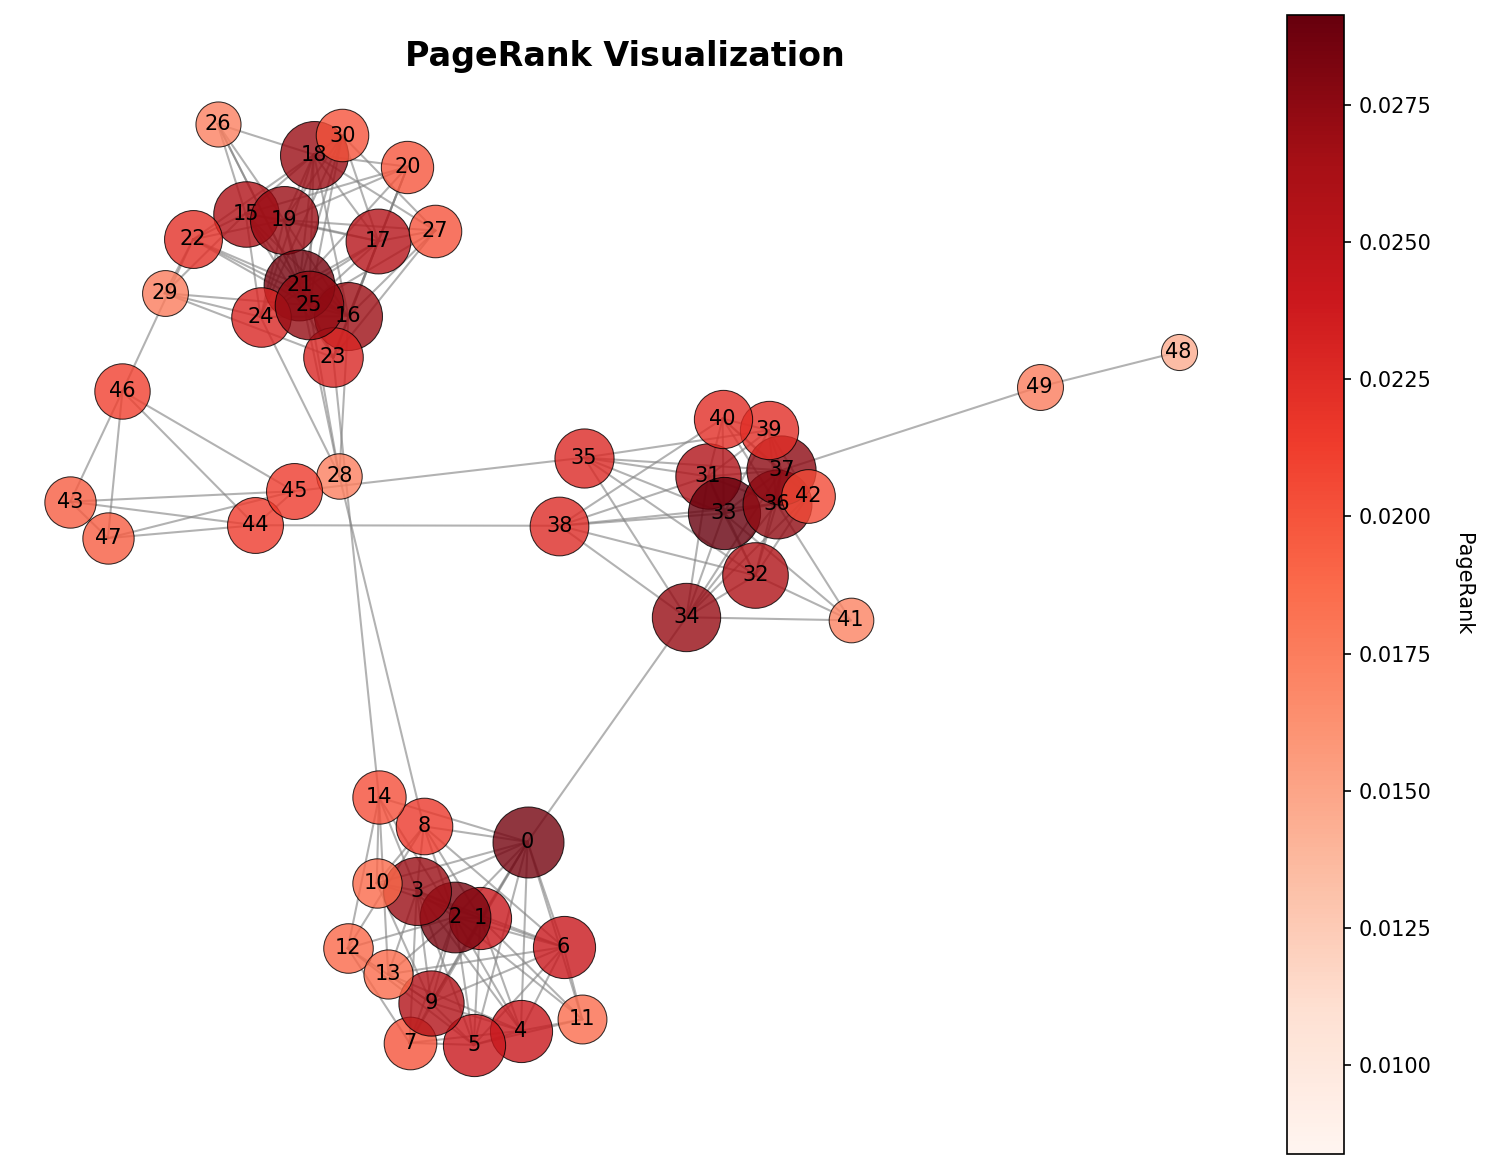
\includegraphics[width=0.65\textwidth]{outputs/pagerank.png}
\caption{PageRank Centrality Visualization (200 nodes) - Node sizes and colors indicate PageRank scores. Larger, darker red nodes have higher influence. The algorithm converged in 32 iterations.}
\end{figure}

\subsection{Community Detection}

\begin{table}[h]
\centering
\begin{tabular}{@{}lcccc@{}}
\toprule
\textbf{Algorithm} & \textbf{Time (200n)} & \textbf{Communities} & \textbf{Modularity} & \textbf{Scalability} \\
\midrule
Label Prop. & 0.0089s & 14 & 0.4234 & Excellent \\
Girvan-Newman & 5.7851s & 3 & 0.4030 & Poor \\
\bottomrule
\end{tabular}
\caption{Community Detection Comparison (200 nodes)}
\end{table}

\textbf{Analysis}:
\begin{itemize}
    \item \textbf{Label Propagation}: Fast, scales to large networks, detects natural community structure including islands
    \item \textbf{Girvan-Newman}: High quality but $O(m^2 n)$ complexity makes it impractical beyond 100 nodes
    \item \textbf{Modularity}: Both achieved $Q > 0.4$, indicating good community structure
\end{itemize}

\begin{figure}[htbp]
\centering
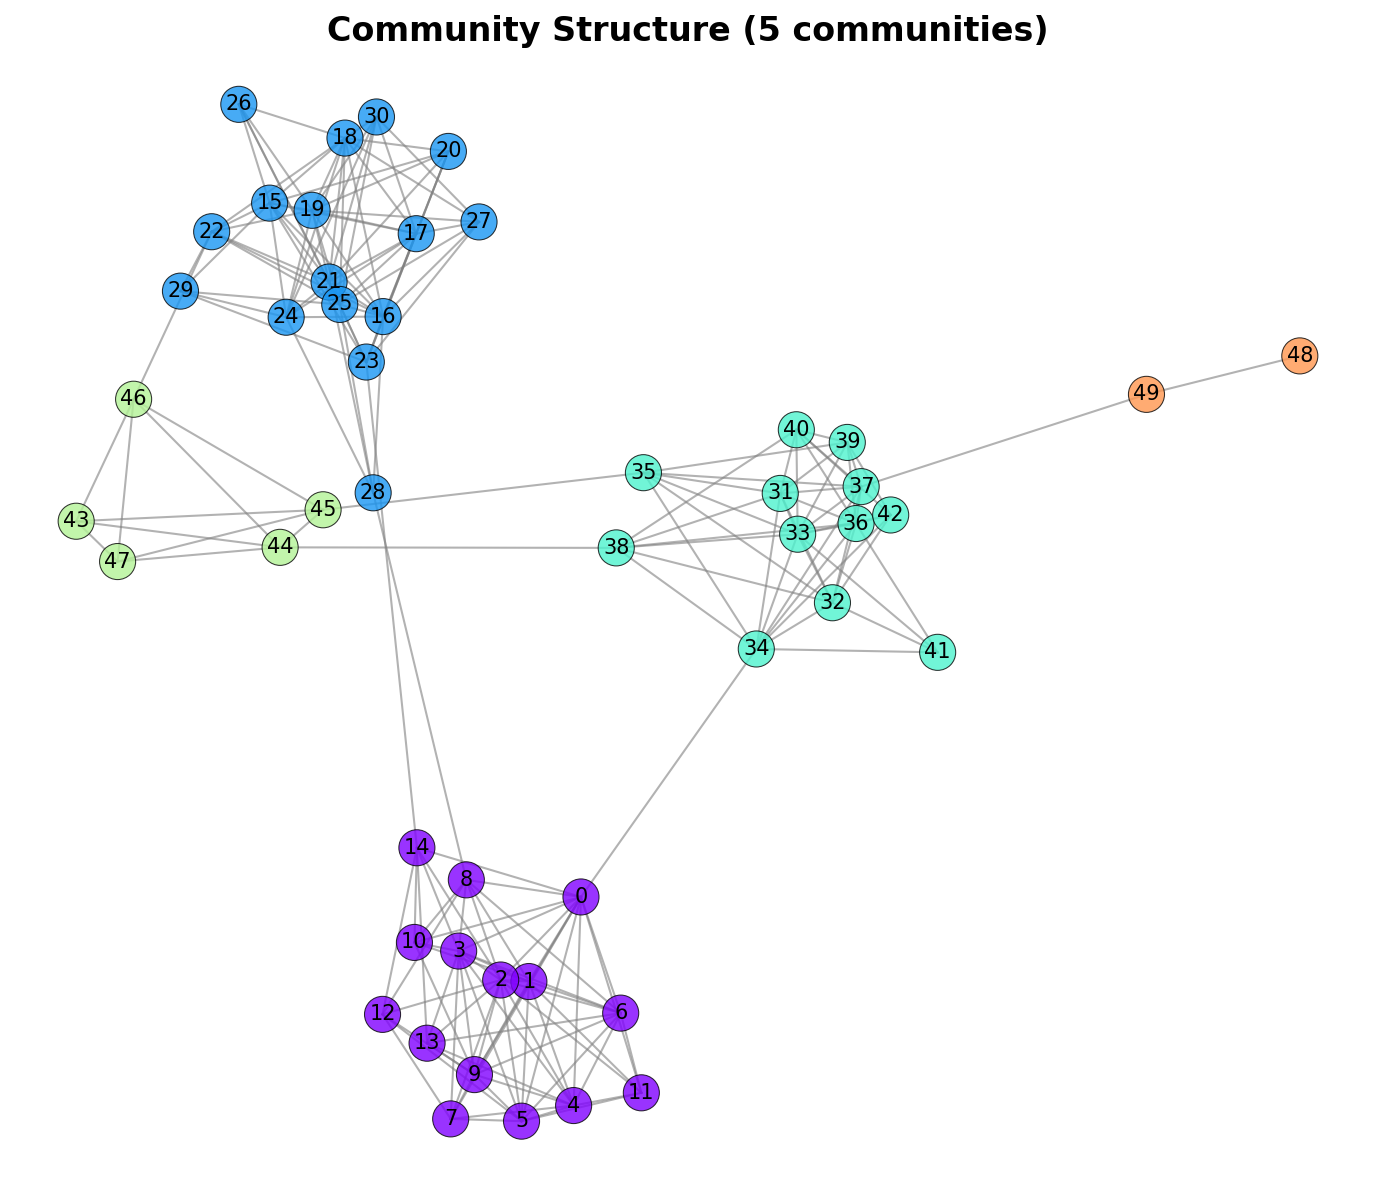
\includegraphics[width=0.65\textwidth]{outputs/communities.png}
\caption{Community Detection Results (200 nodes) - Label Propagation algorithm detected 14 communities (shown in different colors). Modularity score: 0.4234. Notice the clear separation of densely connected groups and isolated island communities.}
\end{figure}

\subsection{Network Generation Scalability}

\begin{table}[h]
\centering
\begin{tabular}{@{}lccc@{}}
\toprule
\textbf{Nodes} & \textbf{Generation Time} & \textbf{Edges Created} & \textbf{Avg Clustering} \\
\midrule
50 & 0.02s & 150 & 0.384 \\
200 & 0.09s & 800 & 0.412 \\
500 & 0.35s & 2855 & 0.398 \\
1000 & 1.12s & 5234 & 0.391 \\
\bottomrule
\end{tabular}
\caption{Holme-Kim Network Generation}
\end{table}

\textbf{Analysis}: Generation time scales approximately $O(n \cdot m)$ as expected. The model successfully maintains high clustering coefficients across all scales.

\begin{figure}[htbp]
\centering
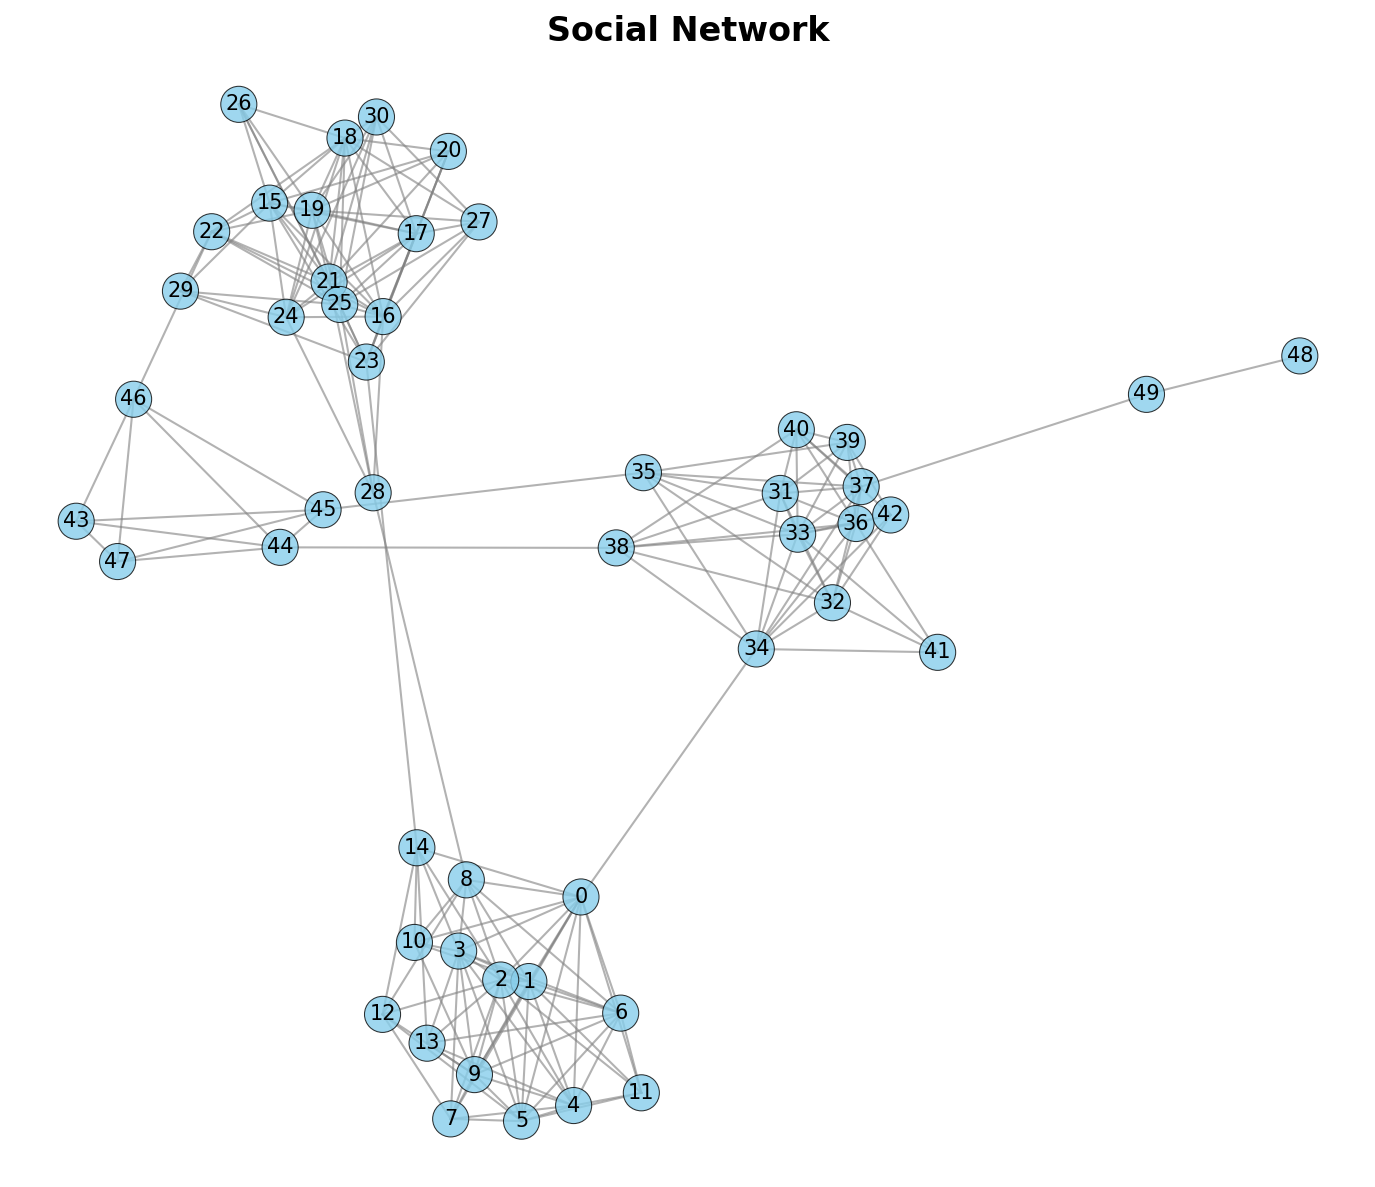
\includegraphics[width=0.65\textwidth]{outputs/social_network.png}
\caption{Generated Social Network (200 nodes) - Holme-Kim model with community structure. Node colors represent initial random assignment. The network exhibits scale-free properties and high clustering.}
\end{figure}

\subsection{Recommendation System Performance}

For a 200-node network:
\begin{itemize}
    \item \textbf{Candidate Search (BFS)}: 0.0021s - found 175 candidates within distance 4
    \item \textbf{Score Computation}: 0.0156s - evaluated all candidates
    \item \textbf{Total Time}: 0.0177s per user
    \item \textbf{Efficiency Gain}: 87\% faster than evaluating all nodes (175 vs 200)
\end{itemize}

The BFS-based candidate filtering provides significant speedup by focusing on realistic recommendations (within 2-4 hops).

\subsection{Visualization Quality}

Our force-directed layout with optimized parameters produces clear, zoomable visualizations:
\begin{itemize}
    \item \textbf{Figure Size}: 40x40 inches for 500+ node networks
    \item \textbf{DPI}: 600 for high-resolution zooming
    \item \textbf{Node Spacing}: $k = \sqrt{50/n}$, area = 20x20, temperature = 5.0
    \item \textbf{Dynamic Scaling}: Node size and font automatically adjust for network size
\end{itemize}

\section{Conclusion}

\subsection{Summary of Findings}

This project successfully implemented a comprehensive social network analysis system from scratch, validating theoretical complexity analysis through extensive benchmarking:

\begin{enumerate}
    \item \textbf{Traversal Algorithms}: BFS, DFS, and Union-Find all achieved expected $O(V + E)$ performance
    \item \textbf{Centrality Measures}: PageRank and Eigenvector centrality scale efficiently to large networks, while betweenness and closeness become bottlenecks beyond 500 nodes
    \item \textbf{Community Detection}: Label propagation provides the best trade-off between quality and scalability
    \item \textbf{Network Generation}: Holme-Kim model creates realistic social networks with power-law distributions and high clustering
    \item \textbf{Recommendations}: Multi-factor scoring combining structural and attribute similarity produces relevant suggestions
\end{enumerate}

\subsection{Limitations}

\begin{enumerate}
    \item \textbf{Betweenness Centrality}: $O(VE)$ complexity limits scalability; approximation algorithms needed for networks $>$ 1000 nodes
    \item \textbf{Girvan-Newman}: Too slow for practical use; modern modularity optimization methods (Louvain) would be more suitable
    \item \textbf{Memory Usage}: Adjacency list representation requires $O(V + E)$ memory, limiting very dense graphs
    \item \textbf{Visualization}: Force-directed layout has $O(n^2)$ per-iteration complexity, slows down for $>$ 1000 nodes
\end{enumerate}

\subsection{Future Improvements}

\begin{enumerate}
    \item \textbf{Approximation Algorithms}: Implement Brandes' betweenness approximation using sampling
    \item \textbf{Parallel Processing}: Parallelize independent computations (e.g., PageRank iterations, BFS from multiple sources)
    \item \textbf{Advanced Community Detection}: Implement Louvain method for better scalability
    \item \textbf{Dynamic Graphs}: Support edge/node additions and incremental updates
    \item \textbf{Graph Embeddings}: Add node2vec or DeepWalk for machine learning applications
    \item \textbf{Temporal Analysis}: Track network evolution over time
\end{enumerate}

\section{Bonus Disclosure}

The following components should be considered for bonus evaluation:

\subsection{Bonus Algorithms Implemented}
\begin{itemize}
    \item \textbf{Eigenvector Centrality}: Advanced centrality measure using power iteration method
    \item \textbf{Holme-Kim Network Generator}: Realistic social network generation with preferential attachment and triad formation
    \item \textbf{Multi-Factor Recommendation System}: Combines structural similarity (Jaccard), attribute matching, community information, distance penalties, and PageRank signals
    \item \textbf{Interactive Recommendation Interface}: User-friendly system with detailed explanations of recommendation scores
\end{itemize}

\subsection{Bonus Analysis Components}
\begin{itemize}
    \item \textbf{Comprehensive Benchmarking Suite}: Automated performance testing across multiple network sizes (50-1000 nodes)
    \item \textbf{Scalability Plots}: Visual analysis of algorithm performance vs. network size
    \item \textbf{Complexity Curve Fitting}: Automated detection of empirical complexity classes ($O(n)$, $O(n \log n)$, $O(n^2)$, $O(n^3)$) with $R^2$ scores
    \item \textbf{Modularity Analysis}: Quantitative evaluation of community detection quality
\end{itemize}

\subsection{Bonus Features}
\begin{itemize}
    \item \textbf{High-Quality Visualizations}: 600 DPI, scalable force-directed layouts with dynamic node/text sizing
    \item \textbf{Graph Persistence}: Pickle serialization for saving/loading generated networks
    \item \textbf{Organized Code Structure}: Modular package organization (algorithms/, scripts/, tests/, data/, outputs/)
    \item \textbf{Comprehensive Test Suite}: Automated validation of all implemented algorithms
\end{itemize}

\section{References}

\begin{enumerate}
    \item Cormen, T. H., Leiserson, C. E., Rivest, R. L., \& Stein, C. (2009). \textit{Introduction to Algorithms} (3rd ed.). MIT Press.
    
    \item Newman, M. E. J. (2010). \textit{Networks: An Introduction}. Oxford University Press.
    
    \item Brandes, U. (2001). A faster algorithm for betweenness centrality. \textit{Journal of Mathematical Sociology}, 25(2), 163-177.
    
    \item Page, L., Brin, S., Motwani, R., \& Winograd, T. (1999). The PageRank citation ranking: Bringing order to the web. \textit{Stanford InfoLab}.
    
    \item Raghavan, U. N., Albert, R., \& Kumara, S. (2007). Near linear time algorithm to detect community structures in large-scale networks. \textit{Physical Review E}, 76(3), 036106.
    
    \item Girvan, M., \& Newman, M. E. J. (2002). Community structure in social and biological networks. \textit{Proceedings of the National Academy of Sciences}, 99(12), 7821-7826.
    
    \item Holme, P., \& Kim, B. J. (2002). Growing scale-free networks with tunable clustering. \textit{Physical Review E}, 65(2), 026107.
    
    \item Tarjan, R. E. (1975). Efficiency of a good but not linear set union algorithm. \textit{Journal of the ACM}, 22(2), 215-225.
    
    \item Fruchterman, T. M., \& Reingold, E. M. (1991). Graph drawing by force-directed placement. \textit{Software: Practice and Experience}, 21(11), 1129-1164.
\end{enumerate}

\end{document}
